
\section{PID}
El algoritmo \textbf{PID} está compuesto por una parte proporcional, integral y derivativa.

\begin{equation}
  u(t) = K_c \left[ e(t) + \frac{1}{T_i} \int_{0}^{t} e(\tau) d\tau + T_d \frac{de(t)}{dt} \right] 
  \label{eq:pid_continuo}
\end{equation}

Para proteger los actuadores mecánicos de la planta (bombas) de los cambios bruscos inducidos por el operador, se implementa la \textbf{derivada sobre la variable de proceso (PV)}. Sabiendo que $e(t) = SP(t) - PV(t)$ y asumiendo un SP constante durante el cálculo de la derivada ($\frac{dSP}{dt} = 0$), se reemplaza $\frac{de(t)}{dt}$ por $-\frac{dPV(t)}{dt}$. La ecuación a discretizar resulta:

\begin{equation}
  u(t) = \underbrace{K_c e(t)}_{P} + \underbrace{\frac{K_c}{T_i} \int_{0}^{t} e(\tau) d\tau}_{I} - \underbrace{K_c T_d \frac{dPV(t)}{dt}}_{D} + u_{bias}
  \label{eq:pid_continuo_mod}
\end{equation}

Para implementar esta ley en el entorno de tiempo real del PLC (\textit{Texto Estructurado}), con un tiempo de muestreo constante $T_s$, se emplean aproximaciones numéricas.

\clearpage

\subsection{PID industrial}

El diagrama \textbf{PID} industrial comprende los parámetros
\begin{itemize}
  \item Switch de accionamiento
  \item Switch derivativo
  \item Saturación
  \item Rate limiter
  \item Switch Automático manual
  \item Switch Remoto local
  \item Noise band
\end{itemize}

\begin{figure}[H]
  \begin{center}
    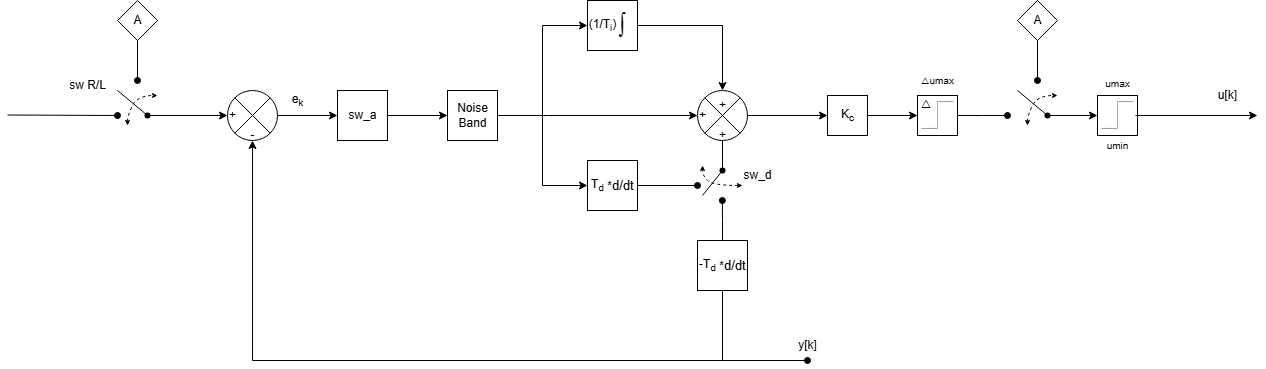
\includegraphics[width=0.8\textwidth]{figures/PIDindustrial.png}
  \end{center}
  \caption{PID industrial}\label{fig:PIDindustrial}
\end{figure}

\subsection{PID discreto}
Para poder discretizar el algoritmo de control, existen 3 métodos principales para poder aproximar los términos integral y derivativo.


\subsubsection{Aproximación Trapezoidal}
La Aproximación trapezoidal asume una interpolación lineal del error entre la muestra anterior y la actual, calculando el área de un trapecio. Es numéricamente más estable y preciso:
\begin{figure}[H]
  \begin{center}
    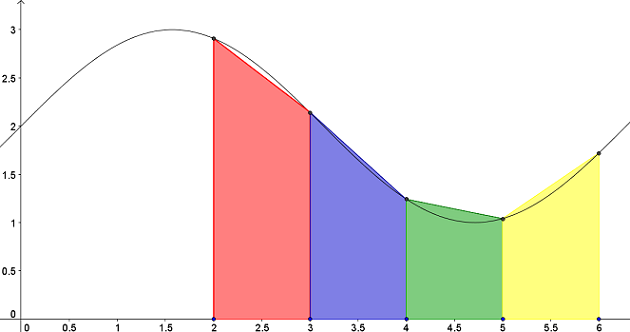
\includegraphics[width=0.7\textwidth]{figures/trapecio.png}
  \end{center}
  \caption{Aproximación trapezoidal}\label{trap-ejemplo}
\end{figure}

\begin{equation}
  \int_{0}^{t} e(\tau) d\tau \approx T_s\sum_{i=1}^{k}\frac{e_i+e_{i-1}}{2}
  \label{trapezoidal}
\end{equation}
Luego reemplazando la ecuación \ref{trapezoidal} en la ecuación del \textbf{PID} 
\[
  u_k = K_c [e_k + \frac{T_s}{2T_i}[\sum_{i=0}^{k}(e_i + e_{i-1})] + T_d(\frac{e_k - e_{k-1}}{T_s})]
\]

\[
  u_k = K_c [e_k(1 + \frac{T_d}{T_s}) + e_{k}(-\frac{T_d}{T_s}) + \frac{T_s}{2T_i}\sum_{i=0}^{k}(e_i + e_{i-1})]
\]

Luego, se repite para $u_{k-1}$

\[
  u_{k-1} K_c [e_{k-1} + \frac{T_s}{2T_i}[\sum_{i=0}^{k-1}(e_i + e_{i-1})] + T_d(\frac{e_{k-1} - e_{k-2}}{T_s})]
\]

\[
  u_{k-1} = K_c [e_{k-1}(1 + \frac{T_d}{T_s}) + e_{k-2}(-\frac{T_d}{T_s}) + \frac{T_s}{2T_i}\sum_{i=0}^{k-1}(e_i + e_{i-1})]
\]
Finalmente juntando todo

\[
  u_k - u_{k-1} = K_c[e_k(1 + \frac{T_d}{T_s}) + e_{k-1}(-1 - \frac{2T_d}{T_s}) + e_{k-2}(\frac{T_d}{T_s}) + \frac{T_s}{2T_i}(e_k + e_{k-1})]
\]
\begin{equation}
  \Delta u_k = e_k\underbrace{K_c(1 + \frac{T_s}{2T_i} + \frac{T_d}{T_s})}_{q_0} + e_{k-1}\underbrace{K_c(-1 + \frac{T_s}{2T_i} - \frac{2T_d}{T_s})}_{q_1} + e_{k-2}\underbrace{K_c(\frac{T_d}{T_s})}_{q_2})]
  \label{PID-trapecio}
\end{equation}

\subsubsection{Aproximación Rectangular (Euler Hacia Atrás)}
La aproximación de Euler hacia atrás (o Backward Euler) asume que el error se mantiene constante en el valor actual durante todo el intervalo de muestreo, calculando el área de un rectángulo hacia la izquierda. Es computacionalmente más eficiente y garantiza estabilidad al mapear el semiplano izquierdo continuo dentro del círculo unitario discreto.


\begin{equation}
  \int_{0}^{t} e(\tau) d\tau \approx T_s\sum_{i=1}^{k} e_i
  \label{euler-atras}
\end{equation}

Reemplazando la ecuación \ref{euler-atras} en la ley de control PID (y utilizando la diferencia finita hacia atrás para la derivada):
\[
  u_k = K_c \left[ e_k + \frac{T_s}{T_i}\sum_{i=1}^{k}e_i + T_d\left(\frac{e_k - e_{k-1}}{T_s}\right) \right]
\]

Luego, se evalúa para el instante anterior $u_{k-1}$:
\[
  u_{k-1} = K_c \left[ e_{k-1} + \frac{T_s}{T_i}\sum_{i=1}^{k-1}e_i + T_d\left(\frac{e_{k-1} - e_{k-2}}{T_s}\right) \right]
\]

Restando ambas expresiones ($u_k - u_{k-1}$) para obtener la forma de velocidad (incremental), la diferencia de las sumatorias se reduce únicamente al término actual $e_k$:
\[
  u_k - u_{k-1} = K_c \left[ (e_k - e_{k-1}) + \frac{T_s}{T_i}e_k + \frac{T_d}{T_s}(e_k - 2e_{k-1} + e_{k-2}) \right]
\]

Finalmente, agrupando por los términos de error actual y pasados:
\begin{equation}
  \Delta u_k = e_k\underbrace{K_c\left(1 + \frac{T_s}{T_i} + \frac{T_d}{T_s}\right)}_{q_0} + e_{k-1}\underbrace{K_c\left(-1 - \frac{2T_d}{T_s}\right)}_{q_1} + e_{k-2}\underbrace{K_c\left(\frac{T_d}{T_s}\right)}_{q_2}
  \label{PID-euler-atras-final}
\end{equation}

\vspace{1cm}

\subsubsection{Aproximación Rectangular (Euler Hacia Adelante)}
La aproximación de Euler hacia adelante (o Forward Euler) calcula el área del rectángulo utilizando el valor del error en el instante anterior. Aunque es matemáticamente intuitiva, presenta problemas de inestabilidad si el tiempo de muestreo $T_s$ es elevado.

\begin{equation}
  \int_{0}^{t} e(\tau) d\tau \approx T_s\sum_{i=0}^{k-1} e_i
  \label{euler-adelante}
\end{equation}

Sustituyendo la ecuación \ref{euler-adelante} en el PID. Nótese que la acción derivativa se mantiene con la aproximación hacia atrás ($\frac{e_k - e_{k-1}}{T_s}$) para preservar la causalidad del controlador, dado que no es posible predecir el error futuro $e_{k+1}$:
\[
  u_k = K_c \left[ e_k + \frac{T_s}{T_i}\sum_{i=0}^{k-1}e_i + T_d\left(\frac{e_k - e_{k-1}}{T_s}\right) \right]
\]

Para el instante anterior $u_{k-1}$:
\[
  u_{k-1} = K_c \left[ e_{k-1} + \frac{T_s}{T_i}\sum_{i=0}^{k-2}e_i + T_d\left(\frac{e_{k-1} - e_{k-2}}{T_s}\right) \right]
\]

Al restar $u_k - u_{k-1}$, la diferencia entre ambas sumatorias deja como residuo el término del instante anterior $e_{k-1}$:
\[
  u_k - u_{k-1} = K_c \left[ (e_k - e_{k-1}) + \frac{T_s}{T_i}e_{k-1} + \frac{T_d}{T_s}(e_k - 2e_{k-1} + e_{k-2}) \right]
\]

Factorizando y definiendo los coeficientes polinomiales $q$:
\begin{equation}
  \Delta u_k = e_k\underbrace{K_c\left(1 + \frac{T_d}{T_s}\right)}_{q_0} + e_{k-1}\underbrace{K_c\left(-1 + \frac{T_s}{T_i} - \frac{2T_d}{T_s}\right)}_{q_1} + e_{k-2}\underbrace{K_c\left(\frac{T_d}{T_s}\right)}_{q_2}
  \label{PID-euler-adelante-final}
\end{equation}
